\documentclass[11pt]{article}
\usepackage{geometry}
\usepackage{graphicx}
\usepackage{enumitem}
\usepackage{array}
\usepackage{multicol}

\geometry{a4paper, top=0.5in, bottom=0.5in, right=0.75in, left=0.75in}
\renewcommand{\arraystretch}{1.5}

\title{Sequential Logic}
\author{Abanoub Emad Hanna}
\date{}

\begin{document}

\maketitle

\section*{Important Definitions}
\subsection*{Combinational vs Sequential}
\begin{itemize}
    \item \textbf{Combinational Logic:} Output depends only on the current input.
    \item \textbf{Sequential Logic:} Output depends on the current and previous inputs, thus it has memory.
\end{itemize}

\subsection*{Static vs Dynamic}
\begin{itemize}
    \item \textbf{Combinational Logic:}
        \begin{itemize}
            \item Static: No clock input.
            \item Dynamic: Clock input is required.
        \end{itemize}
    \item \textbf{Sequential Logic:}
        \begin{itemize}
            \item Static: Feedback used to retain output indefinitely.
            \item Dynamic: Temporary charge on a capacitor.
        \end{itemize}
\end{itemize}

\subsection*{Synchronous vs Asynchronous}
\begin{itemize}
    \item \textbf{Synchronous:} Clock-driven.
    \item \textbf{Asynchronous:} Event-driven.
\end{itemize}


\section*{Latches}
Latches are level-sensitive devices. Data passes only when transparent and is stored when opaque.
\subsection*{Types}
\begin{itemize}
    \item \textbf{Positive Latch:}
        \begin{itemize}
            \item Transparent when CLK is high.
            \item Setup \& hold times are defined at the negative edge of CLK.
        \end{itemize}   
    \item \textbf{Negative Latch:}
        \begin{itemize}
            \item Transparent when CLK is low.
            \item Setup \& hold times are defined at the positive edge of CLK.
        \end{itemize}
    \item \textbf{Note:}
    Setup \& hold times are defined when we are going to store the input, so in the case of a positive-edge triggered FF, setup \& hold times are defined at the positive edge of CLK. In the case of a positive latch, we want to store when opaque, so setup \& hold times are defined at the negative edge of CLK.
\end{itemize}

\pagebreak

\subsection*{Design}
\subsubsection*{Dynamic Latch}
\begin{multicols}{2}
    \begin{minipage}{0.9\linewidth}
        \begin{center}
            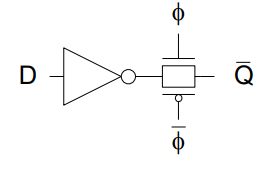
\includegraphics[width=0.8\textwidth]{dynamic_latch.png}
        \end{center}
    \end{minipage}
    \begin{minipage}{\linewidth}
        \begin{center}
            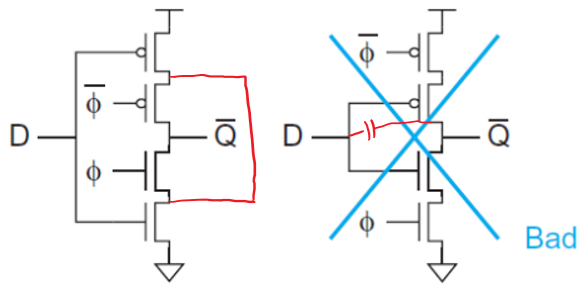
\includegraphics[scale=0.6]{latch2.png}
        \end{center}
    \end{minipage}
\end{multicols}
\noindent
If the red wire is removed, this topology is known as $C^2MOS$ latch, which is immune to clock skew. Second topology is bad due to the capactior between the output and the input.


\subsubsection*{Static Latch}
    \begin{minipage}{0.5\linewidth}
        \begin{itemize}
            \item Buffered input and ouptut so no backdriving.
            \item large and slightly slow but very robust.
            \item High clock loading.
            \item Recommended for all but performance- or area-critical designs
        \end{itemize}
    \end{minipage}
    \hfill
    \begin{minipage}{0.4\linewidth}    
        \begin{center}
            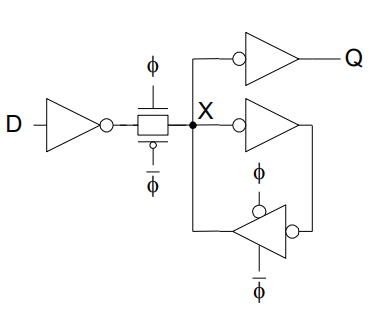
\includegraphics[width=0.8\textwidth]{latch3.png}
        \end{center}
    \end{minipage}

\section*{Flip-Flops}
Flip-Flops are (+ve or -ve) edge-triggered devices. Data passes only at the edge of the clock signal and stored till the next cycle.

\subsection*{Design}
Master-slave configuration is the most popular. For a positive-edge triggered FF, the master is negative latch and the slave is positive latch. When clock is low, master is transparent (captures the input) and slave is opaque (holds old value; ouptut = $Q_n$). When clock is high, slave latch is transparent (ouptut = D).\\
\textbf{Note:} Slave latch controls the ouptut, so it is same type as the FF.

\begin{multicols}{2}
    \subsubsection*{MUX-Based}
    \begin{minipage}{\linewidth}
        \begin{center}
            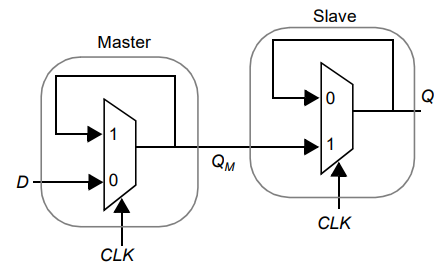
\includegraphics[width=0.8\textwidth]{MUX.png}
        \end{center}
    \end{minipage}
    \subsubsection*{Standard FF}
    \begin{minipage}{\linewidth}
        \begin{center}
            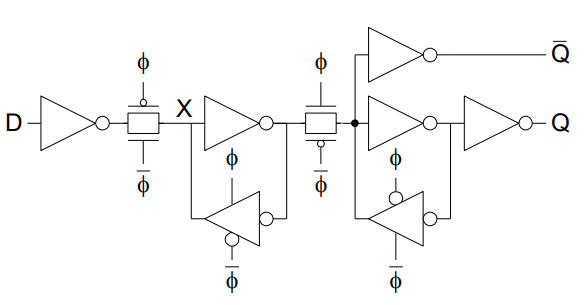
\includegraphics[width=0.8\textwidth]{PTL.png}
        \end{center}
    \end{minipage}
\end{multicols}

\pagebreak

\subsection*{Types}
\begin{multicols}{2}

\subsubsection*{D Flip-Flop}
    \begin{minipage}{\linewidth}
        \begin{center}
            $Q_{n+1} = D$
        \end{center}
    \end{minipage}

\subsubsection*{SR Flip-Flop}
    \begin{minipage}{\linewidth}
        \begin{center}
            \begin{tabular}{ |c|c|c| } 
                \hline
                S & R & $Q_{n+1}$ \\
                \hline
                0 & 0 & $Q_n$ \\
                \hline
                0 & 1 & 0 \\
                \hline
                1 & 0 & 1 \\
                \hline
                1 & 1 & X \\
                \hline
            \end{tabular}
        \end{center}
    \end{minipage}

\subsubsection*{JK Flip-Flop}
    \begin{minipage}{\linewidth}
        \begin{center}
            \begin{tabular}{ |c|c|c| } 
                \hline
                J & K & $Q_{n+1}$ \\
                \hline
                0 & 0 & $Q_n$ \\
                \hline
                0 & 1 & 0 \\
                \hline
                1 & 0 & 1 \\
                \hline
                1 & 1 & $\overline{Q_n}$ \\
                \hline
            \end{tabular}
        \end{center}
    \end{minipage}

\subsubsection*{T Flip-Flop}
    \begin{minipage}{\linewidth}
        \begin{center}
            \begin{tabular}{ |c|c| } 
                \hline
                T & $Q_{n+1}$ \\
                \hline
                0 & $Q_n$ \\
                \hline
                1 & $\overline{Q_n}$ \\
                \hline
            \end{tabular}
        \end{center}
    \end{minipage}
\end{multicols}

\subsection*{Type Conversion}
\textbf{Steps:}
\begin {enumerate}
    \item Construct truth table for the desired FF.
    \item Add $Q_n$ column if converting from D or T.
    \item Fill the values of the current FF's truth table depending on the ouput.
    \item Use K-Maps or intuition to simplify the equations.
\end {enumerate}

\begin{multicols}{2}
\subsubsection*{SR to D}
    \begin{minipage}{\linewidth}
        \begin{center}
            \begin{tabular}{ |c|c|c|c| } 
                \hline
                D & S & R & $Q_{n+1}$ \\
                \hline
                0 & 0 & 1 & 0\\
                \hline
                1 & 1 & 0 & 1 \\
                \hline
            \end{tabular}\\
            \vspace{10pt}
            $S=D$ \& R=$\overline{D}$
        \end{center}
    \end{minipage}
\subsubsection*{JK to T}
    \begin{minipage}{\linewidth}
        \begin{center}
            \begin{tabular}{ |c|c|c|c| } 
                \hline
                T & J & K & $Q_{n+1}$ \\
                \hline
                0 & 0 & 0 & $Q_n$\\
                \hline
                1 & 1 & 1 & $\overline{Q_n}$ \\
                \hline
            \end{tabular}\\
            \vspace{10pt}
            $J=T$ \& R=$K=T$
        \end{center}
    \end{minipage}
\subsection*{D to JK}
    \begin{minipage}{\linewidth}
        \begin{center}
            \begin{tabular}{ |c|c|c|c|c|c| } 
                \hline
                J & K & $Q_n$ & D & $Q_{n+1}$ \\
                \hline
                0 & 0 & 0 & 0 & 0\\
                \hline
                0 & 0 & 1 & 1 & 1\\
                \hline
                0 & 1 & 0 & 0 & 0\\
                \hline
                0 & 1 & 1 & 0 & 0\\
                \hline
                1 & 0 & 0 & 1 & 1\\
                \hline
                1 & 0 & 1 & 1 & 1\\
                \hline
                1 & 1 & 0 & 1 & 1\\
                \hline
                1 & 1 & 1 & 0 & 0\\
                \hline
            \end{tabular}\\
            \vspace{10pt}
            $D=J\overline{Q_n}+\overline{K}Q_n$
        \end{center}
    \end{minipage}
\end{multicols}

\section*{Frequency Dividers}
\begin{center}
    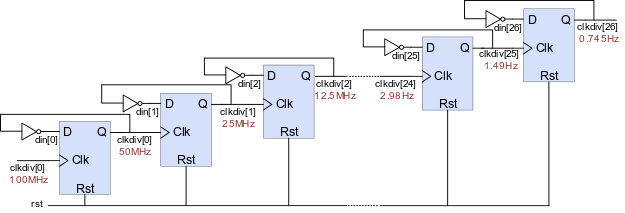
\includegraphics[scale=0.7]{clk1.png}
\end{center}
Frequency divider can also be done by making T = 1 for T FF and J = K = 1 for JK FF.

\section*{Counter}
\begin{center}
    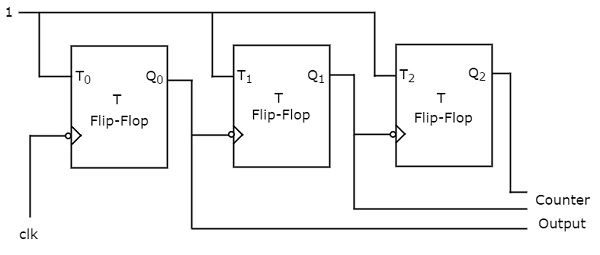
\includegraphics[width=0.9\linewidth]{counter.jpg}
\end{center}

\noindent
\begin{minipage}[t]{0.55\textwidth}
    \vspace*{-90pt}
    \begin{itemize}
        \item We try to find any patterns in the truth table.
        \item Q0 toggles every clock cycle, so we set \(T = 1\) for the first FF.
        \item Q1 toggles only at the falling edge of Q0, so we set \(T = 1\) and invert the clock for the second FF.
        \item Q2 toggles only at the falling edge of Q1, so we set \(T = 1\) and invert the clock for the third FF.
    \end{itemize}
\end{minipage}%
\hfill
\begin{minipage}[t]{0.4\textwidth}
    \centering
    \begin{tabular}{|c|c|c|}
        \hline
        Q2 & Q1 & Q0 \\
        \hline
        0 & 0 & 0 \\
        0 & 0 & 1 \\
        0 & 1 & 0 \\
        0 & 1 & 1 \\
        1 & 0 & 0 \\
        1 & 0 & 1 \\
        1 & 1 & 0 \\
        1 & 1 & 1 \\
        \hline
    \end{tabular}
\end{minipage}


\end{document}
